\documentclass[12pt,a4paper]{article}
\usepackage{amssymb}
%\usepackage{latexsym}
\usepackage{amsmath}
\usepackage{listings}
\usepackage{graphicx}
\usepackage{color}
\usepackage{url}

% Stolen settings (unknown origin):
% Alter some LaTeX defaults for better treatment of figures:
% See p.105 of "TeX Unbound" for suggested values.
% See pp. 199-200 of Lamport's "LaTeX" book for details.
%   General parameters, for ALL pages:
\renewcommand{\topfraction}{0.9}	% max fraction of floats at top
\renewcommand{\bottomfraction}{0.8}	% max fraction of floats at bottom
%   Parameters for TEXT pages (not float pages):
\setcounter{topnumber}{2}
\setcounter{bottomnumber}{2}
\setcounter{totalnumber}{4}     % 2 may work better
\setcounter{dbltopnumber}{2}    % for 2-column pages
\renewcommand{\dbltopfraction}{0.9}	% fit big float above 2-col. text
\renewcommand{\textfraction}{0.07}	% allow minimal text w. figs
%   Parameters for FLOAT pages (not text pages):
\renewcommand{\floatpagefraction}{0.7}	% require fuller float pages
% N.B.: floatpagefraction MUST be less than topfraction !!
\renewcommand{\dblfloatpagefraction}{0.7}	% require fuller float pages

% remember to use [htp] or [htpb] for placement

\author{Rasmus Einarsson, Jonatan Kallus, Olof Nilsson, Joel Wilsson}
\title{Simulation of Complex Systems\\Lattice gas automata}

\begin{document}
\maketitle

\section{Introduction}
Lattice gas automata are a kind of cellular automata, which are used to model some aspects of the physics of gases, such as diffusion and waves.

This text explores the behaviour of lattice gas automata. A number of simulations are run to qualitatively see if the model captures some phenomena expected from actual gases. The investigated phenomena are specifically waves, diffusion and currents of a flow around a cylinder. Some attempts are made to make meaningful comparisons to the theory of gas physics.

The theory of lattice gas automata in general is introduced in section~\ref{sec:theory} followed by the specific details of our implementation in section~\ref{sec:imp}. The conducted experiments and their results are presented in section~\ref{sec:exp}. In the last section, section~\ref{sec:conclusion}, we conclude that the model can capture waves and diffusion, but not the typical behaviour of a compressed flow around a cylinder. There, we also discuss the benefits and disadvantages of the model.

Cellular automata in general, thus also lattice gas automata, are systems that are discrete in time and in space. They are built using a small set of deterministic rules, usually a mapping from each possible spatial configuration of some small area into a spatial configuration of that area for the next time step.

The mayor benefit of simulation of gases using lattice gas automata is simplicity, the model is built using only simple rules. The simulations does not require any differential equations to be solved, neither explicitly nor implicitly. The scientific interest in lattice gas automata declined drastically in the beginning of the 1990-ties, probably due to the increased interest in more sophisticated models using Lattice Boltzmann methods. The new models made it possible to capture more of the phenomena of fluid physics, and were made possible by faster computers.

\section{Theory}
\label{sec:theory}

\section{Implementation details}
\label{sec:imp}
% describe bouncing off walls, random initializations at sources... anything else?

\section{Experiments, results}
\label{sec:exp}
% or should this just say ``waves''?
\subsection{Shockwaves}
We start out with a square area, surrounded by walls, where initially each lattice site (not including walls)
is completely filled with a probability of 0.3. Completely filled means that it contains six or
four particles, if we use a hexagonal or a square lattice, respectively. After one time step,
this looks completely random, as can be seen in figure \ref{hexwaveinit}. In this figure, and the
next few figures, we used a hexagonal lattice. The effects of using a square lattice instead will be
explained in the last part of this section.

\begin{figure}[htp]
% if we change to just waves, this caption needs to be changed.
\caption{Initial conditions, after one time step, for the shockwave experiment using a hexagonal lattice.}
\centering
  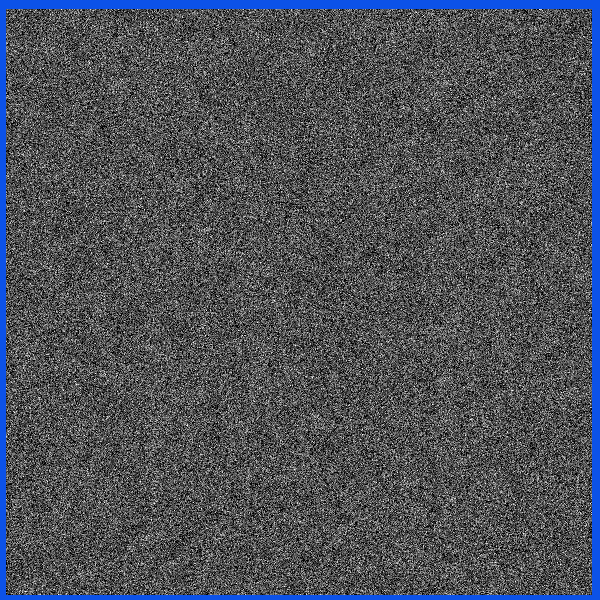
\includegraphics[width=100pt]{figs/hexwaveinit.png}
\label{hexwaveinit}
\end{figure}

By clicking the left mouse button we set a circular area of lattice sites around the mouse cursor to
be completely filled. Just like a real gas, on average these added particles move towards areas of lower
concentrations of particles, away from the spawn point (since the circular area has the highest concentration
possible). Three frames taken just after the particles were added are shown in figure \ref{hexwavestart}.

\begin{figure}[htp]
\caption{Frames demonstrating the initial phase of the shockwave.}
\centering
  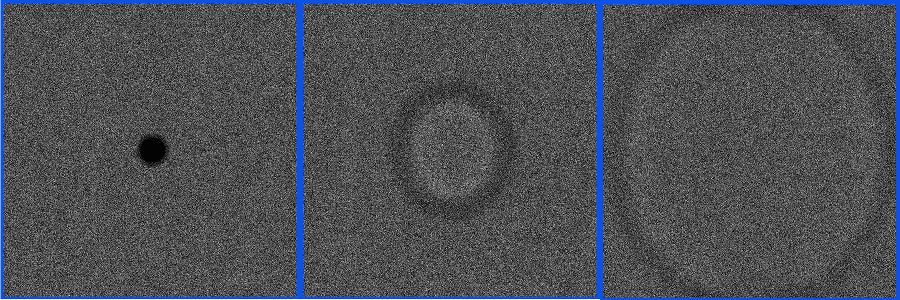
\includegraphics[width=300pt]{figs/hexwavestart.png}
\label{hexwavestart}
\end{figure}


The resulting waves bounce off against the walls, figure \ref{hexwavebounce}.
\begin{figure}[htp]
\caption{Just like real waves, the lattice gas shockwaves bounce off the walls.}
\centering
  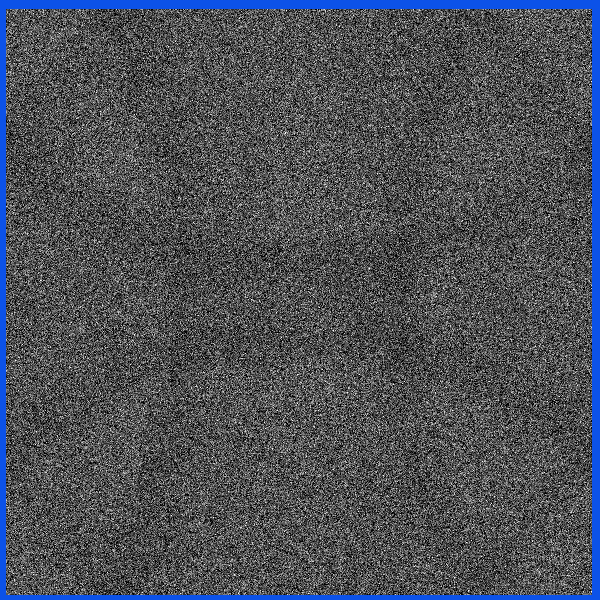
\includegraphics[width=100pt]{figs/hexwavebounce.png}
\label{hexwavebounce}
\end{figure}

Eventually, through collisions
with the other random particles in the box, the particles we added spread out and the pattern which was formed
when we filled the circular area is lost. Figure \ref{hexwaveend} shows what it looks like many time
steps later (approximately 30 seconds later, when the simulation is run on a fast computer).
We can see no trace of the shockwave.

\begin{figure}[htp]
\caption{Many updates later, the picture looks the same as before the shockwave.}
\centering
  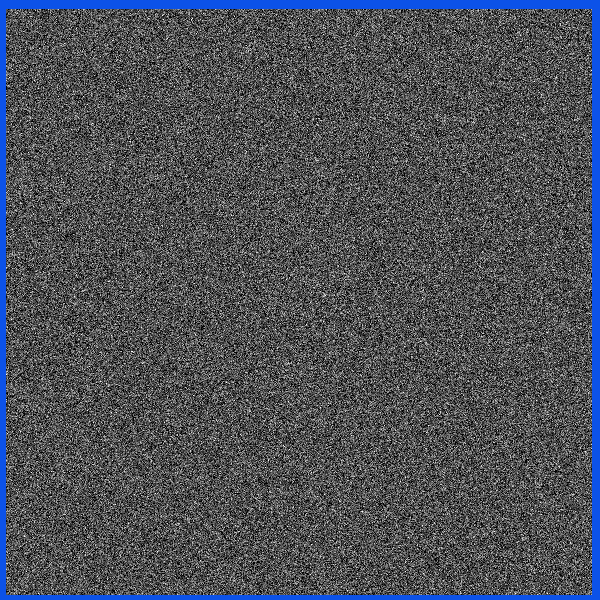
\includegraphics[width=100pt]{figs/hexwaveend.png}
\label{hexwaveend}
\end{figure}


% compare to analytical results, if possible?

If we use a square lattice instead, we still get the wave-like behaviour, figure \ref{squarewave}.
\begin{figure}[htp]
\caption{The shockwave looks similar when using a square lattice.}
\centering
  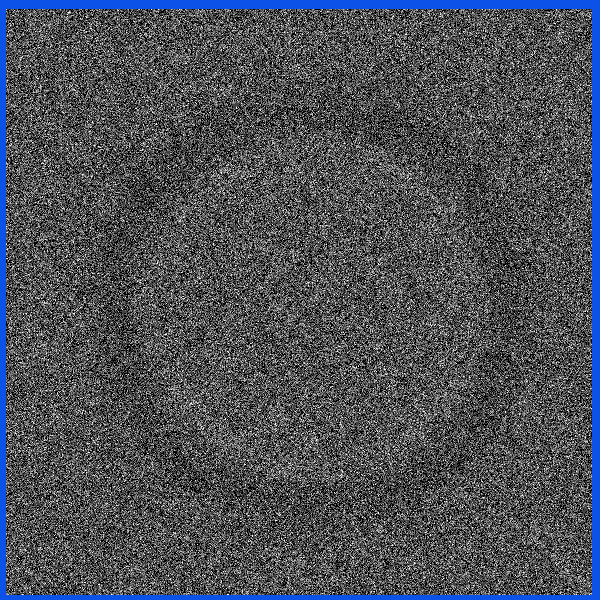
\includegraphics[width=100pt]{figs/squarewave.png}
\label{squarewave}
\end{figure}

However, the waves persist for much longer, possibly because there are fewer possible collisions.
Even after letting the simulation run for a long time after the particles were added, traces of waves
going back and forth can still be seen. Unfortunately, this is not clear from a static picture, so
it's not possible to show them in this report.

% the following is a hypothesis. it makes sense to me, but does it make sense to you?
Also, there are fewer particles in total (since each site can contain at most four particles, instead of six).
This means there are fewer possible states for the system, and therefore it has lower entropy, so patterns
(such as the non-randomly initialized circle completely filled with particles) which lower the entropy would make
a bigger relative difference than for the hexagonal lattice.

\subsection{Diffusion}
In this experiment, we have three boxes in a row, and the gas can spread between adjacent boxes through a small
hole in the separating wall. Initially, all boxes are empty except for the first one, where each lattice site
is completely filled with particles. The initial conditions are shown in figure \ref{diffusioninit}.

\begin{figure}[htp]
% if we change to just waves, this caption needs to be changed.
\caption{Initial conditions, after one time step, for the diffusion experiment.}
\centering
  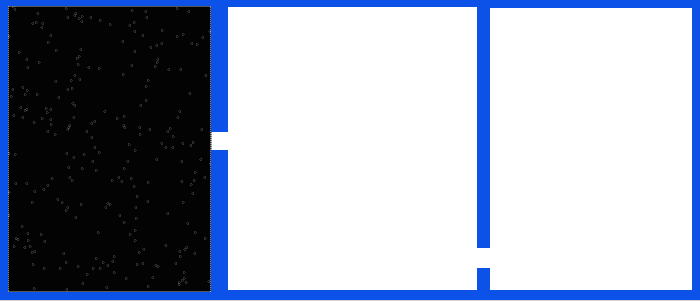
\includegraphics[width=200pt]{figs/diffusioninit.png}
\label{diffusioninit}
\end{figure}

As the simulation runs, the gas spreads first to the second box (figure \ref{diffusionbox2fill}.
\begin{figure}[htp]
\caption{Much of the gas has spread to the second box.}
\centering
  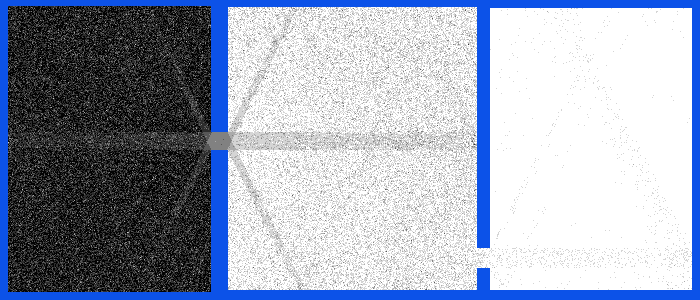
\includegraphics[width=200pt]{figs/diffusionbox2fill.png}
\label{diffusionbox2fill}
\end{figure}

Eventually, particles also start to fill up the third box (figure \ref{diffusionbox3fill}.
\begin{figure}[htp]
\caption{A while later, many particles are also found in the third box.}
\centering
  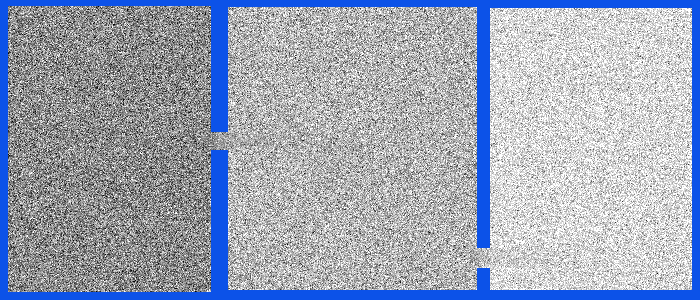
\includegraphics[width=200pt]{figs/diffusionbox3fill.png}
\label{diffusionbox3fill}
\end{figure}

Given enough time, they spread out uniformly over the whole available space, just like a real gas would.
This ``steady-state'' is shown in figure \ref{diffusionend}.
\begin{figure}[htp]
\caption{Eventually, the particle density is the same for all boxes.}
\centering
  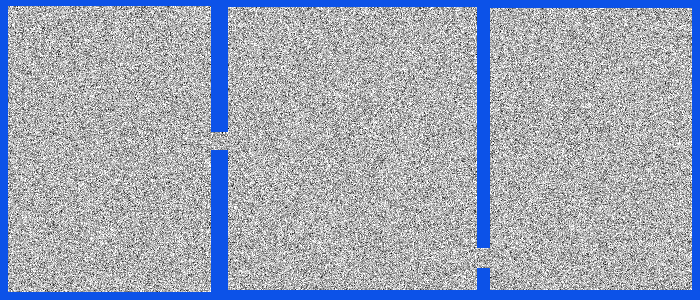
\includegraphics[width=200pt]{figs/diffusionend.png}
\label{diffusionend}
\end{figure}

We modified our program to count the number of particles in each box; see figure \ref{gascount}.
% compare to theoretical results?
\begin{figure}[htp]
\caption{Number of particles in each box as a function of the number of updates.}
\centering
  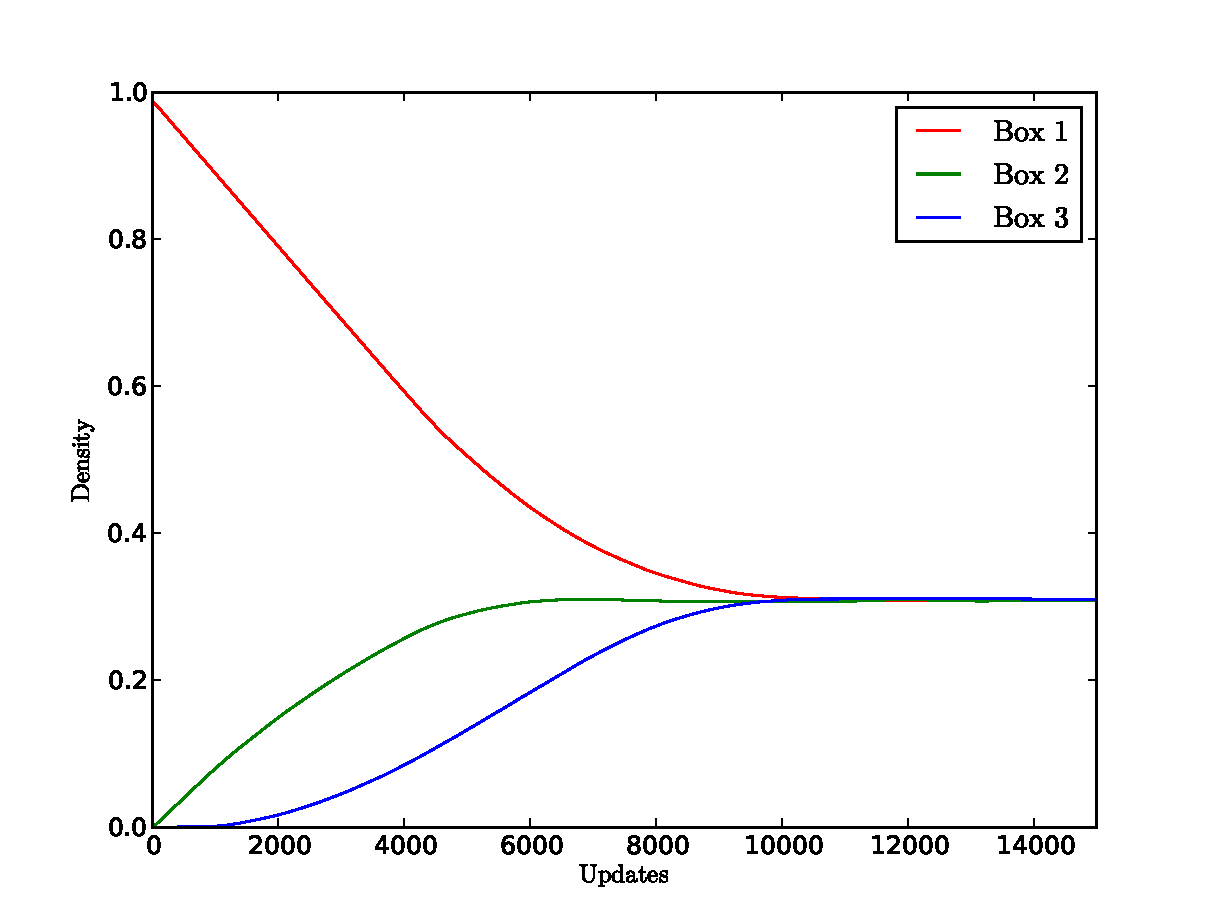
\includegraphics[width=300pt]{figs/gascount.pdf}
\label{gascount}
\end{figure}

\subsection{Flow around cylinder}

\section{Conclusion}
\label{sec:conclusion}

\end{document}
